\chapter{Complete Example (Markus)} \label{sec:Example}

This chapter presents a complete example of a transformation with story diagrams. The setting of the example is explained in Section \ref{sec:Example:Motivation}. The next section then presents several complex story diagrams that the execute the transformation.

\section{Motivation of the example}
\label{sec:Example:Motivation}

One well-known principle of object-oriented programming says \emph{``Program to an interface, not an implementation.''} \cite{GHJV95}. By only accessing interfaces instead of concrete classes from a given class, that class remains independent of concrete implementations. The accessed class can be exchanged transparently without breaking the program. If this principle is neglected, accidentally or intentionally, this is known as an \emph{interface violation}.

\begin{figure}[hbtp]
\centering
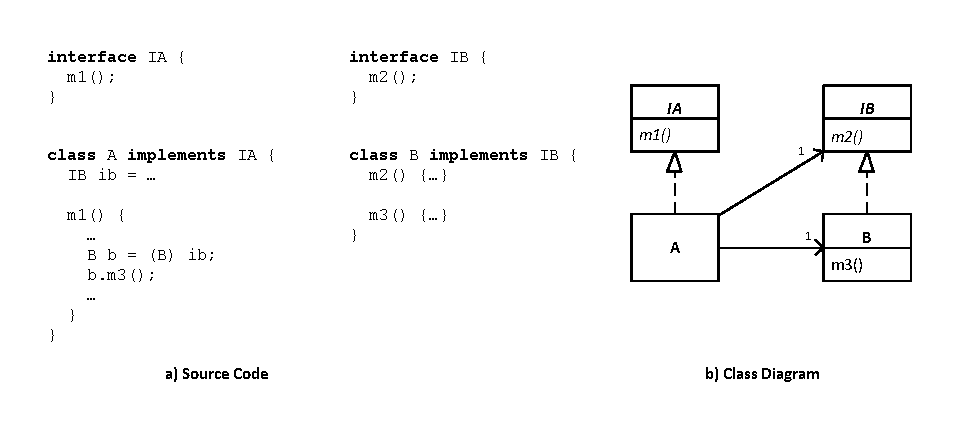
\includegraphics[width=\linewidth]{./figures/InterfaceViolation}
\caption{Example of an interface violation}
\label{fig:InterfaceViolationExample}
\end{figure}

In Figure~\ref{fig:InterfaceViolationExample}, a simple example of an interface violation is depicted. The classes \fe{A} and \fe{B} implement the interfaces \fe{IA} and \fe{IB}, respectively. Following the design principle ``Program to an interface, not an implementation'', the classes are expected to communicate through their interfaces. However, \fe{A} calls the method \fe{m3()} from \fe{B}. Because \fe{m3()} is not provided by the interface \fe{IB}, \fe{A} downcasts the object \fe{ib} to the concrete type \fe{B} in order to access \fe{m3()}. This intentional bypassing of the interface \fe{IB} is an Interface Violation.

There are several possibilities to remove an interface violation from a program. A trivial solution would be to delete the downcast and the call from the implementation \fe{m1}. This would, of course, remove the interface violation but also change the program behavior. A more sensible solution, that will be used in this chapter is the extension of the interface \fe{IB} to contain the method declaration of \fe{m3}. By adding this declaration to \fe{IB}, the class \fe{A} can call \fe{m3} via the interface. The downcast becomes unnecessary and can be removed. At the same time, the behaviour of \fe{m1} is preserved.

To this point, the refactoring is very similar to the \emph{Extract Interface} refactoring described by fowler \cite{Fow99}. Extending an existing interface, however, is a little more complicated as there may already be other classes that implement \fe{IB}. If \fe{m3} is added to \fe{IB}, those other implementing classes all have to be extended by an (possibly empty) method implementation of \fe{m3} in order to remain compilable.

A story diagram that removes an interface violation by extending an interface as described above is presented in the following section.

\section{Story diagram: Remove interface violation}

\begin{figure}[hbtp]
\centering
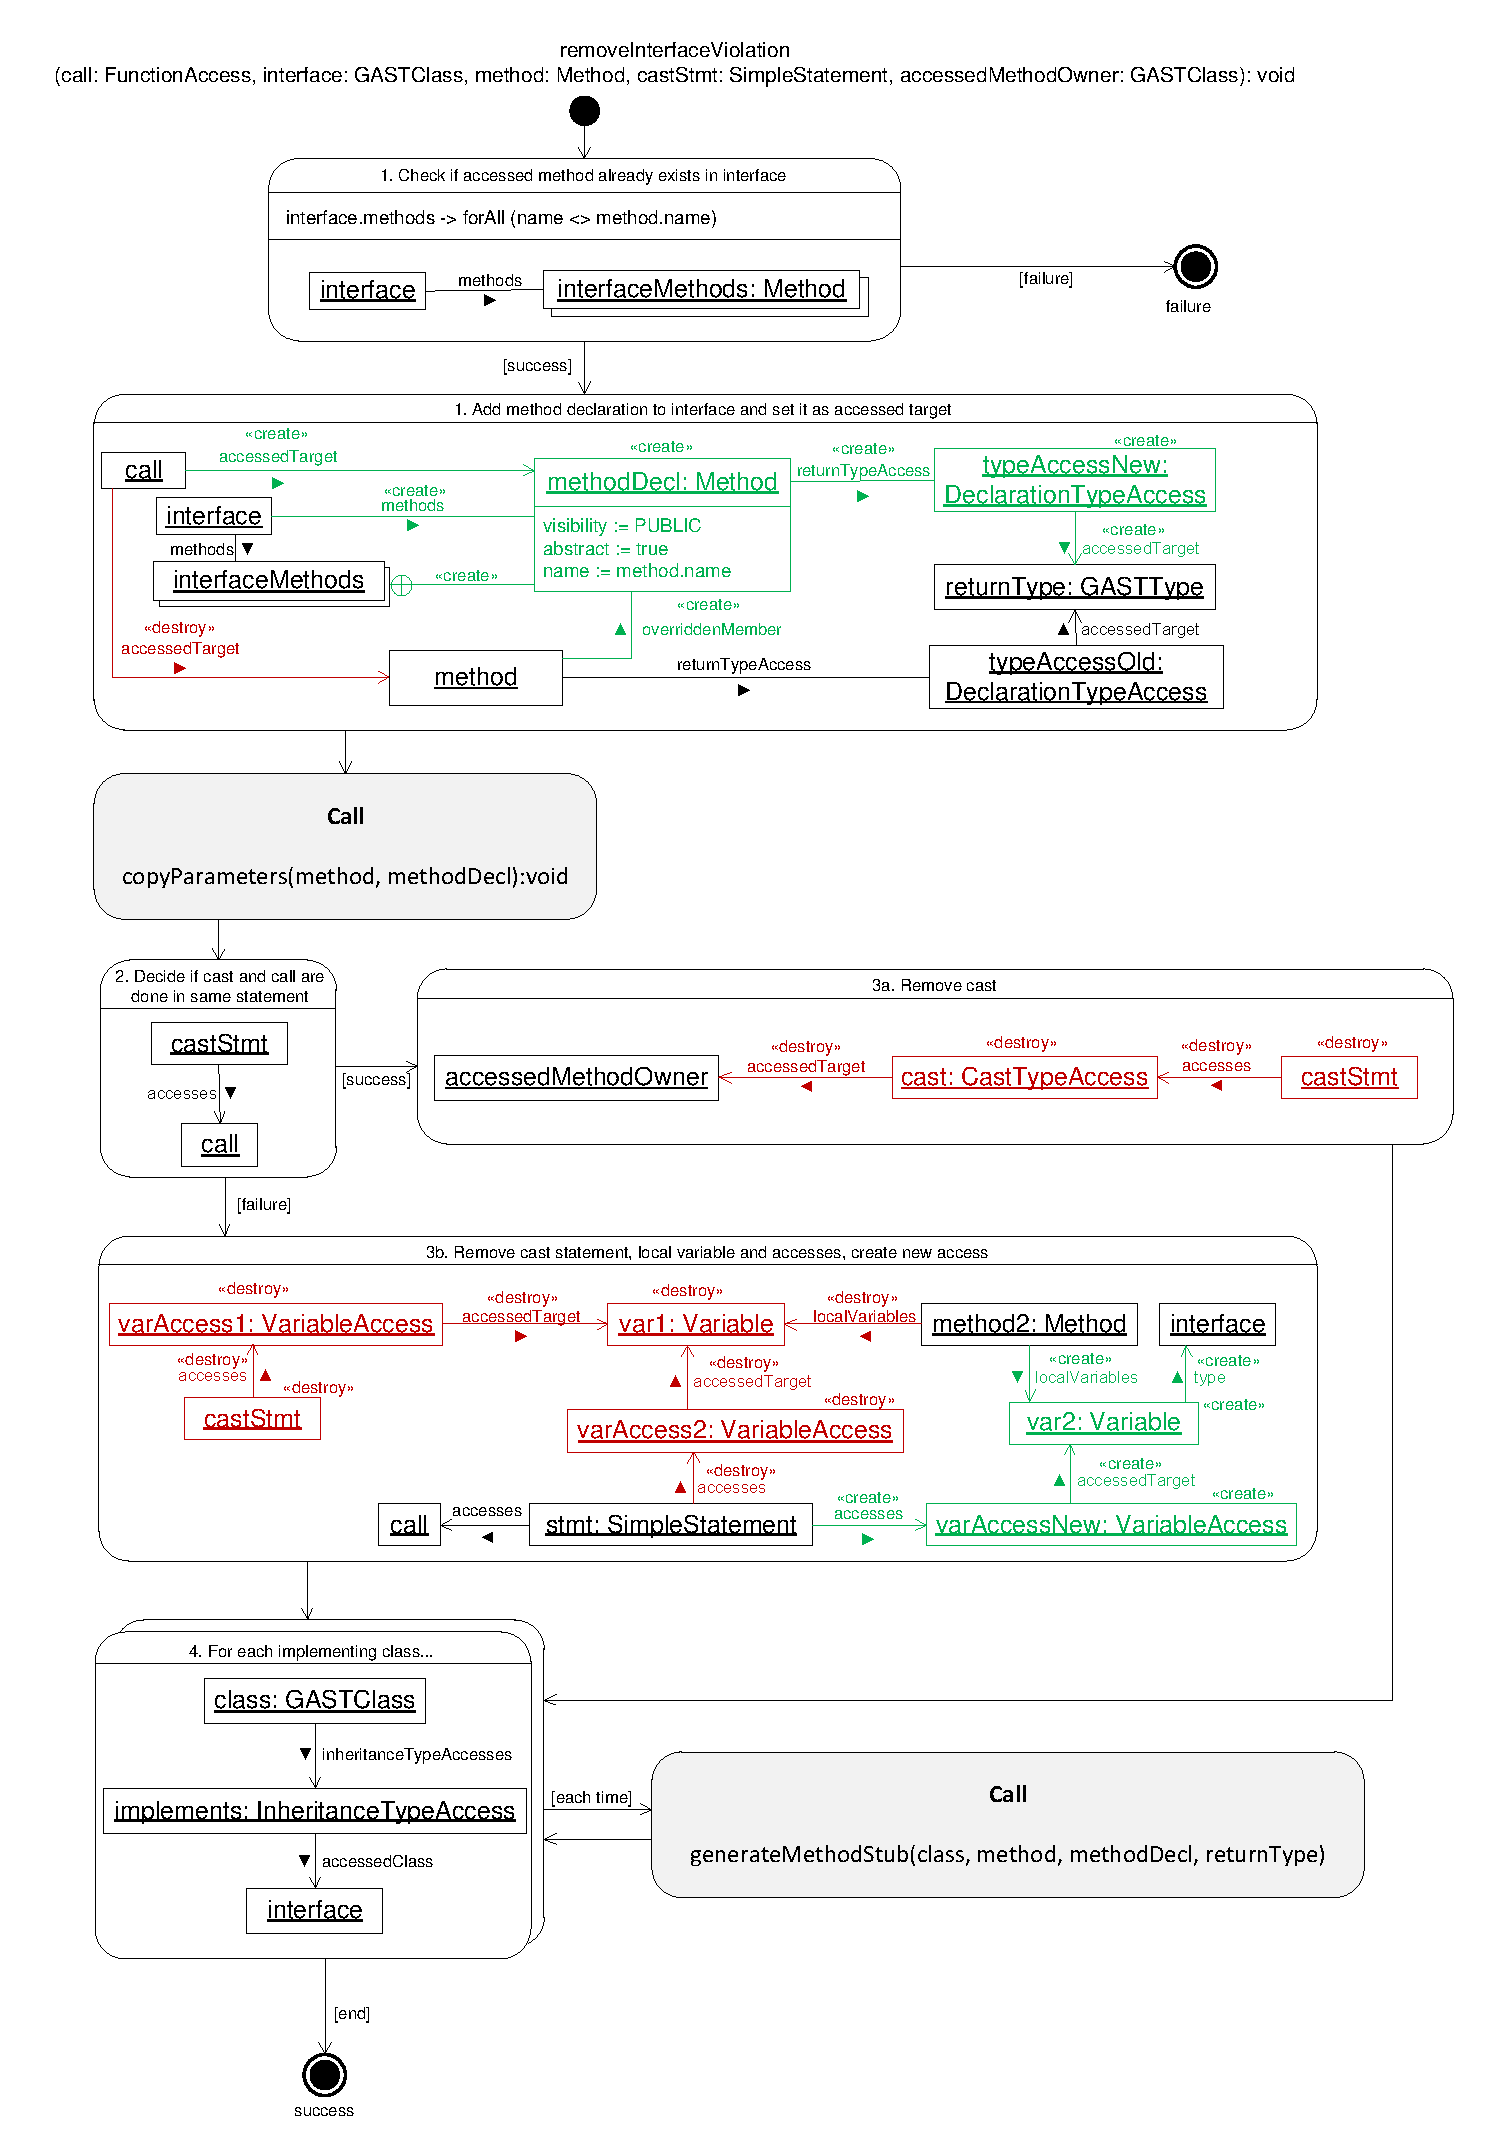
\includegraphics[width=\linewidth]{./figures/SDRemoveInterfaceViolation}
\caption{Story Diagram: RemoveInterfaceViolation}
\label{fig:SDRemoveInterfaceViolation}
\end{figure}

Figure~\ref{fig:SDRemoveInterfaceViolation} shows the story diagram to remove an interface violation. The underlying type graph is the GAST metamodel that was introduced in Section~\ref{sec:typeGraph}. The story diagram consists of five story activities and two activity calls. This section explains the story diagram step by step.

The story diagram has five in-parameters: \fe{call}, \fe{interface}, \fe{method}, \fe{castStmt}, and \fe{accessedMethodOwner}. The \fe{call} represents the statement that calls the method in the concrete class (the call of \fe{m3} in \fe{m1}). The \fe{interface} is the interface that will be extended (\fe{IB} in the example). \fe{method} is the method that is currently not declared in the interface (\fe{m3()}). \fe{castStmt} refers to the statement that down casts the interface type to the concrete class type (i.e., the statement \fe{B b = (B) ib;}). Finally, \fe{accessedMethodOwner} is the class that contains the called \fe{method} (\fe{B} in the example).

The first activity node (after the start node) creates a method declaration in the interface (\fe{methodDecl}). This new method declaration is declared as public (attribute assignment \fe{visibility := PUBLIC}) and abstract (attribute assignment \fe{abstract := true}). The declaration receives the same name as the formerly called method (attribute assignment \fe{name := method.name}, \fe{m3} in the example). The new method declaration is added to the methods of the \fe{interface} by creating a \fe{method} link between \fe{interface} and \fe{methodDecl}. The target accessed by the \fe{call} is changed by deleting the link between \fe{call} and \fe{method} and recreating it between \fe{call} and \fe{methodDecl}. The return type of the method is set by creating a new object \fe{typeAccessNew} of the type \fe{DeclarationTypeAccess} and connecting it to \fe{methodDecl}. It points to the same \fe{GASTType} as the old declaration type access of the \fe{method}.

The next node is an activity call node. It calls the story diagram \emph{Copy parameters} which is described in detail in Section~\ref{sec:SDCopyParameters}. This story diagram is responsible for copying all the parameters of the formerly called \fe{method} to the newly created declaration \fe{methodDecl}.

The following activity node contains only the two bound, mandatory object variables \fe{castStmt} and \fe{call}. It's responsibility is to try and match the link \fe{accesses} between those object variables. If the link exists that means that the cast and the call are part of the same statement. In that case the matching of the activity node is successful and the control flow continues along the transition labelled with \emph{[success]} to activity node 3a. If the matching fails, i.e., the link does not exist and the cast and the call are therefore not part of the same statement, the activity node is left via the \emph{[failure]} transition. This distinction is necessary because the effort to remove the cast statement is much greater if the cast is not done in the same statement as the call (compare activity nodes 3a and 3b).

If the cast is in the same statement as the call, activity node 3a is executed: The \fe{castStmt} and its access to \fe{B} are deleted. If the cast is not in the same statement as the call that means that the cast has to be executed at some point before the call and the resulting downcast object has to be stored in a temporary variable. That variable is later used as a receiving object for the call. In this case, this temporary variable can be deleted along with the accesses to it from the call and the cast statements. Instead, a new variable of the interface type (\fe{IB} in the example) is created and then accessed by the call statement. In both cases, activity node 4 is executed next.

Activity node 4 is responsible for adapting all other classes that implement the now changed interface. Thus, the node is a for each node that binds a class which is connected to the \fe{interface} in each iteration. For each of those bindings, the node that is reachable via the \fe{[each time]} transition is executed (see Section \ref{sec:StoryDiagrams}). In this case that is a story diagram call of the story diagram \fe{GenerateMethodStub} which is explained in the following section.

\subsection{Story diagram: Generate method stub}

\begin{figure}[hbtp]
\centering
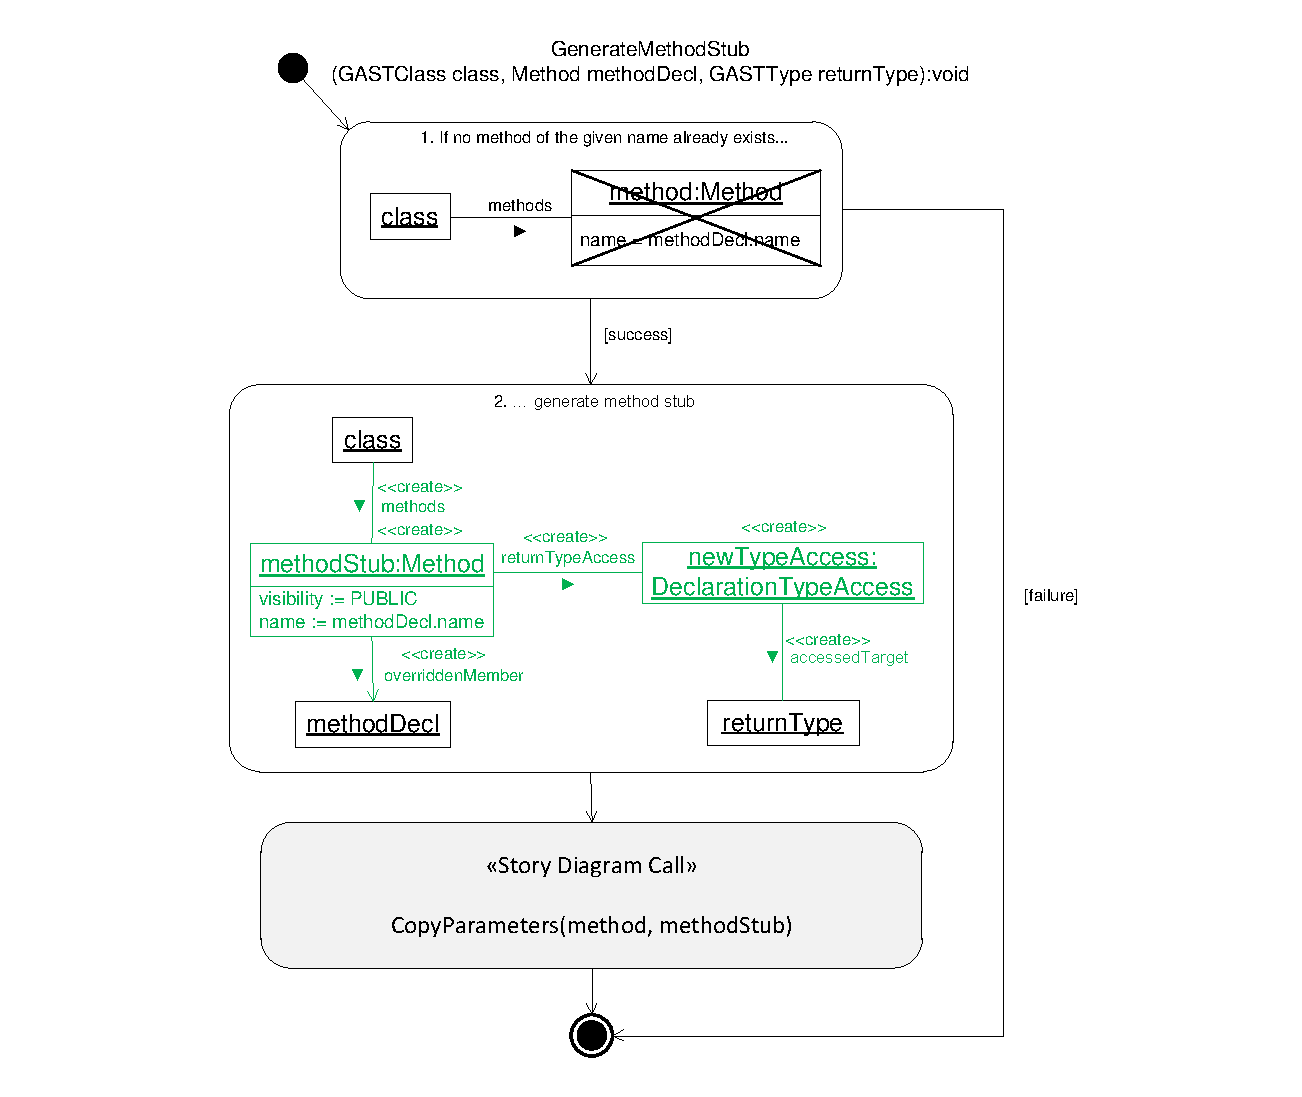
\includegraphics[width=0.9\linewidth]{./figures/SDGenerateMethodStub}
\caption{Story Diagram: GenerateMethodStub}
\label{fig:SDGenerateMethodStub}
\end{figure}

The story diagram \fe{GenerateMethodStub} is shown in Figure~\ref{fig:SDGenerateMethodStub}. It creates a method which implements a method \fe{methodDecl} in a given \fe{interface}. This is accomplished by two activity nodes and one story diagram call. The first node checks if the given \fe{class} contains a \fe{method} with the same name as the given declaration \fe{methodDecl}. The check is performed by the expression \fe{'name = methodDecl.name'}. Since the object variable \fe{method} is negative (crossed-out), the matching of this activity node is considered successful if \emph{no} such method exists in the class. In that case the next activity node is executed. If a method of the name in question already exists, the execution of the first activity node fails and the story diagram terminates.

The second activity node creates a new \fe{methodStub} in the given \fe{class}. The visibility of this method is set to public and its name is set to the name of the method declaration as signified by the expression \fe{'name := methodDecl.name'}. The correct return type for the method is set by creating a \fe{newTypeAccess} from the \fe{methodStub} to the \fe{returnType} that was passed to this story diagram as a parameter.

Finally, the story diagram \fe{CopyParameters} is called in the story diagram call node. The \fe{method} and the \fe{methodStub} are passed as parameters. The called diagram then copies all parameters from the given \fe{method} to the newly created \fe{methodStub}. It is explained in the following section.

\subsection{Story diagram: Copy parameters} \label{sec:SDCopyParameters}

The story diagram \fe{CopyParameters} (see Figure~\ref{fig:SDCopyParameters}) copies all the parameters from a \fe{sourceMethod} to a \fe{targetMethod}. Both methods are provided as parameters. The diagram consists of two activity nodes.

\begin{figure}[hbtp]
\centering
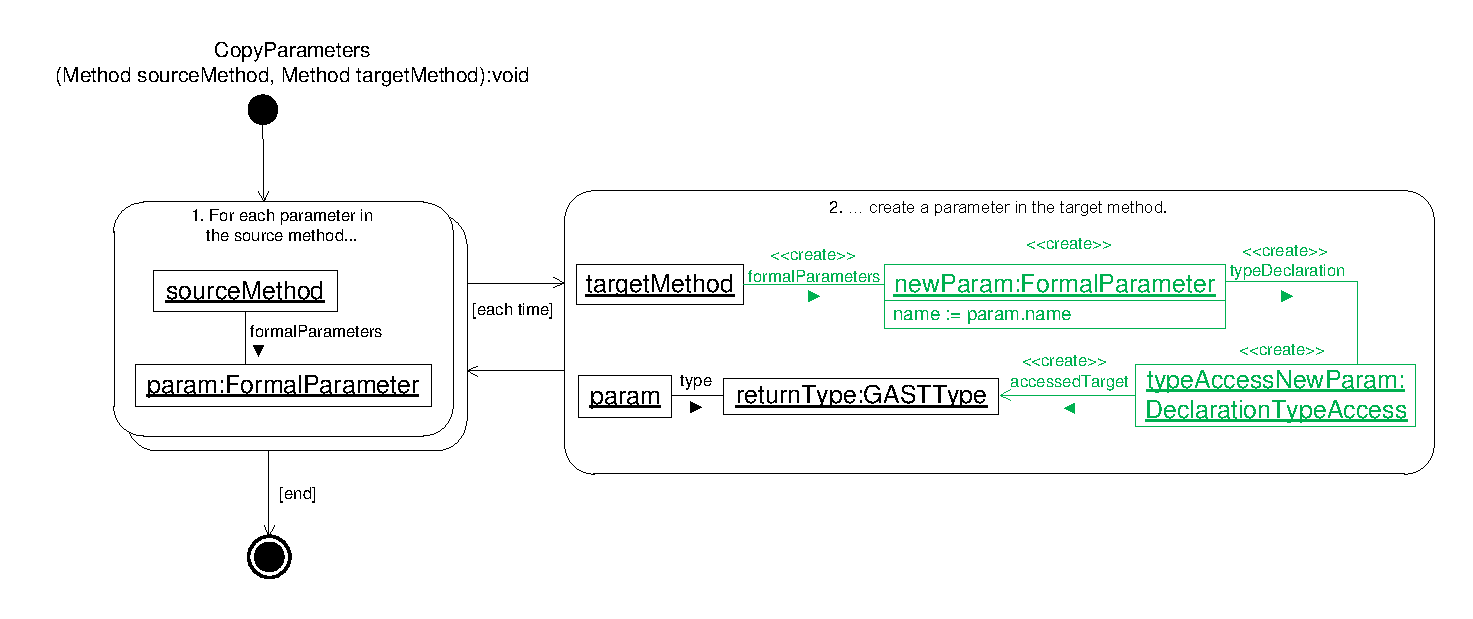
\includegraphics[width=0.9\linewidth]{./figures/SDCopyParameters}
\caption{Story Diagram: CopyParameters}
\label{fig:SDCopyParameters}
\end{figure}

The first activity node is a for each node. It successively binds all formal parameters of the given \fe{sourceMethod} to the object variable \fe{param}. Each time a new parameter is bound, the second activity node is executed. There, a new formal parameter \fe{newParam} is created in the \fe{targetMethod}. Its name is set to the same name as the original parameter's by the expression \fe{'name := param.name'}. The type is also set accordingly by binding the \fe{type} of \fe{param}. Then, a new access to that type is created an connected to \fe{newParam}.